
\begin{center}
\Huge
	Arealformlen og sinusrelationerne
\end{center}

\section*{Arealformlen for vilkårlige trekanter}
\stepcounter{section}

Det er også muligt at bestemme arealet for en trekant, hvis man kender to sider og den mellemliggende vinkel i stedet for højden på trekanten. Denne formel kaldes til tider for \textit{appelsin-formlen}, da formlen lyder lidt som en halv appelsin. Vi betragter trekanten på Figur \ref{fig:vilkårlig}.
\begin{figure}[H]
	\centering
	\begin{tikzpicture}
		\draw[color = olive, thick] (0,0) -- (5,0) node[midway, anchor = north] {$b$};
		\draw[color = olive, thick] (0,0) -- (4,3) node[midway, anchor = south east] {$c$};
		\draw[color = olive, thick] (5,0) -- (4,3) node[midway, anchor = west] {$a$};
		\node[color = olive, anchor = east] at (0,0) {$A$};
		\node[color = olive, anchor = west] at (5,0) {$C$};
		\node[color = olive, anchor = south] at (4,3) {$B$};
	\end{tikzpicture}
	\caption{Vilkårlig trekant $\triangle ABC$}
	\label{fig:vilkårlig}
\end{figure}
For trekanter som denne gælder der følgende sætning
\begin{setn}[Appelsin-formlen]
	\label{setn:areal}
	For vilkårlige trekanter $\triangle ABC$ som den på Figur \ref{fig:vilkårlig} gælder der,
	 at arealet $M$ af trekanten er givet ved
	 \begin{align*}
	 	M = \frac{1}{2}ab \sin(\angle C).
	 \end{align*}
\end{setn}
\begin{proof}
	For at bevise denne sætning, betragter vi følgende trekant $\triangle ABC$.
	\begin{center}
	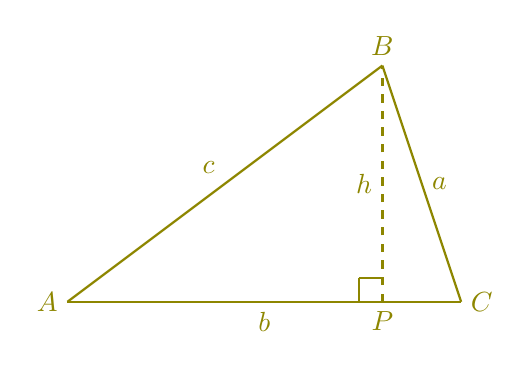
\begin{tikzpicture}
		\draw[color = olive, thick] (0,0) -- (5,0) node[midway, anchor = north] {$b$};
		\draw[color = olive, thick] (0,0) -- (4,3) node[midway, anchor = south east] {$c$};
		\draw[color = olive, thick] (5,0) -- (4,3) node[midway, anchor = west] {$a$};
		\node[color = olive, anchor = east] at (0,0) {$A$};
		\node[color = olive, anchor = west] at (5,0) {$C$};
		\node[color = olive, anchor = south] at (4,3) {$B$};
		\draw[color = olive, thick, dashed] (4,0) -- (4,3) node[midway, anchor = east] {$h$};
		\node[color = olive, anchor = north] at (4,0) {$P$};
		\draw[color = olive, thick] (3.7,0) -- (3.7,0.3);
		\draw[color = olive, thick] (3.7,0.3) -- (4,0.3);
	\end{tikzpicture}
	\end{center}
	Trekant $\triangle BCP$ er en retvinklet trekant med $\angle P = 90^\circ$, så der må gælde, at 
	\begin{align*}
		\sin(\angle C) = \frac{h}{a}.
	\end{align*}
	Vi isolerer $h$ i udtrykket og får
	\begin{align*}
		h = \sin(\angle C)a.
	\end{align*}
	Betragt nu udtrykket for arealet $M$ givet ved
	\begin{align*}
		M = \frac{1}{2}gh.
	\end{align*}
	I trekant $\triangle ABC$ er $g = b$ og vi har lige vist, at $h = \sin(\angle C)a$. Dette indsættes i 
	udtrykket for $M$ og vi får
	\begin{align*}
		M = \frac{1}{2}gh = \frac{1}{2}b\sin(\angle C)a = \frac{1}{2}ab\sin(\angle C).
	\end{align*}
\end{proof}
Vi kan selvfølgelig også navngive hjørnerne i trekanten anderledes. Så fås sætningen som
\begin{align*}
	M = \frac{1}{2}bc\sin(\angle A)
\end{align*}
eller
\begin{align*}
	M = \frac{1}{2}ac\sin(\angle B).
\end{align*}
\begin{exa}
En trekant $\triangle ABC$ er givet ved følgende
\begin{center}
	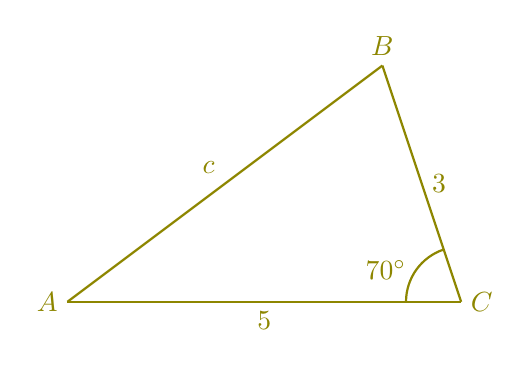
\begin{tikzpicture}
		\draw[color = olive, thick] (0,0) -- (5,0) node[midway, anchor = north] {$5$};
		\draw[color = olive, thick] (0,0) -- (4,3) node[midway, anchor = south east] {$c$};
		\draw[color = olive, thick] (5,0) -- (4,3) node[midway, anchor = west] {$3$};
		\draw[color = olive, thick] (4.3,0) arc (180:180-71.57:0.7) node[midway, anchor = east] {$70^{\circ}$};
		\node[color = olive, anchor = east] at (0,0) {$A$};
		\node[color = olive, anchor = west] at (5,0) {$C$};
		\node[color = olive, anchor = south] at (4,3) {$B$};
	\end{tikzpicture}
\end{center}
For at bestemme arealet, sætter vi ind i formlen. Vi får derfor
\begin{align*}
	M = \frac{1}{2}\cdot 3 \cdot 5 \cdot \sin(70) = 7.05
\end{align*}
og arealet af trekanten er derfor $M = 7.05$.
\end{exa}

Vi skal bruge følgende sætning, når vi skal bevise Sætning \ref{setn:areal} for stumpe vinkler $\angle C$.
\begin{setn}
	\label{setn:cossin}
	For $\cos$ og $\sin$ gælder der, at 
	\begin{align*}
		\cos(v) = -\cos(180 - v),
	\end{align*}
	og
	\begin{align*}
		\sin(v) = \sin(180 - v).
	\end{align*}
\end{setn} 
\begin{proof}
	Opgave
\end{proof}

\section*{Sinusrelationerne}
\stepcounter{section}

Vi kan bruge arealformlen til at sige noget om forholdene mellem vinklerne og sidelængderne i vilkårlige trekanter. Disse forhold kaldes for \textit{sinusrelationerne.}
\begin{setn}[Sinusrelationerne]
	\label{setn:sinusrelation}
	For vilkårlige trekanter $\triangle ABC$ som den på Figur \ref{fig:vilkårlig} gælder der, at 
	\begin{align*}
		\frac{\sin(\angle A)}{a} = \frac{\sin(\angle B)}{b} = \frac{\sin(\angle C)}{c}.
	\end{align*}
\end{setn}
\begin{proof}
	Opgave
\end{proof}

For at se, hvordan sinusrelationerne kan anvendes, ses der på et eksempel.
\begin{exa}
	En trekant er givet ved følgende.
	\begin{center}
		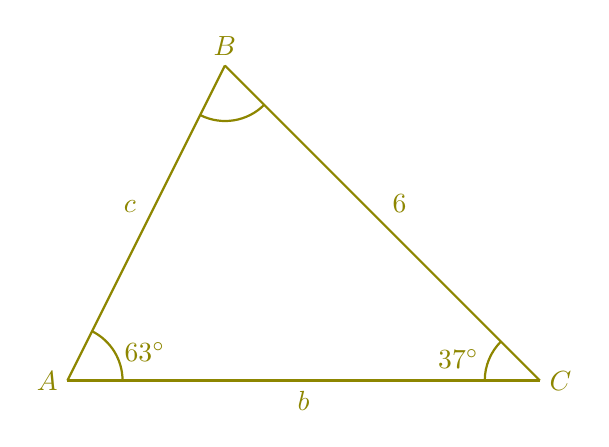
\begin{tikzpicture}
		%A
		\pgfmathsetmacro{\ax}{0}
		\pgfmathsetmacro{\ay}{0}
		%B
		\pgfmathsetmacro{\bx}{2}
		\pgfmathsetmacro{\by}{4}
		%C
		\pgfmathsetmacro{\cx}{6}
		\pgfmathsetmacro{\cy}{0}
		%arc radius
		\pgfmathsetmacro{\arclen}{0.7}
		%c
		\draw[color = olive, thick] (\ax,\ay) -- (\bx,\by) node[midway, anchor = south east] {$c$};
		%b
		\draw[color = olive, thick] (\ax,\ay) -- (\cx,\cy) node[midway, anchor = north] {$b$};
		%a
		\draw[color = olive, thick] (\bx,\by) -- (\cx,\cy) node[midway, anchor = south west] {$6$};
	%	Vinkel A		
		\draw[color = olive, thick] (\ax + \arclen,0) arc (0:63.43:\arclen) 
		node[midway, anchor = west] {$63^{\circ}$};
	%	Vinkel B
		\draw[color = olive, thick] (1.69,3.37) arc (180 + 63.43:180 + 63.43 + 71.57:\arclen)
		 node[midway, anchor = south east] {};
	%	Vinkel C
		\draw[color = olive, thick] (\cx - \arclen,0) arc (180:180 - 45:\arclen)
		 node[midway, anchor = east] {$37^\circ$};
		 %Nodes
		 \node[color = olive, anchor = east] at (\ax,\ay) {$A$};
		 \node[color = olive, anchor = south] at (\bx,\by) {$B$};
		 \node[color = olive, anchor = west] at (\cx,\cy) {$C$};
		\end{tikzpicture}
	\end{center}
	Vi kender $\angle A = 63^\circ$, $\angle C = 37^\circ$ og $a = 6$. Vi kan indsætte dette i 
	sinusrelationerne og får
	\begin{align*}
		\frac{\sin(\angle A)}{a} = \frac{\sin(\angle C)}{c} \Leftrightarrow 
		\frac{\sin(67^\circ)}{6} = \frac{\sin(37^\circ)}{c}
	\end{align*}
	Vi aflæser $\sin(63^\circ) = 0.9$ og $\sin(37^\circ) = 0.6$
	 i Tabel \ref{tab:cossintan} med én decimal.
	Dette indsættes i ligningen og vi får
	\begin{align*}
		\frac{\sin(67^\circ)}{6} = \frac{\sin(37^\circ)}{c} &\Leftrightarrow	
		\frac{0.9}{6} = \frac{0.6}{c} \\
		&\Leftrightarrow	 c = \frac{6\cdot 0.6}{0.9} = \frac{3.6}{0.9} = 4,
	\end{align*}
	og derfor er $c = 4$. 
\end{exa} 

\newpage


\begin{table}[H]
	\centering
	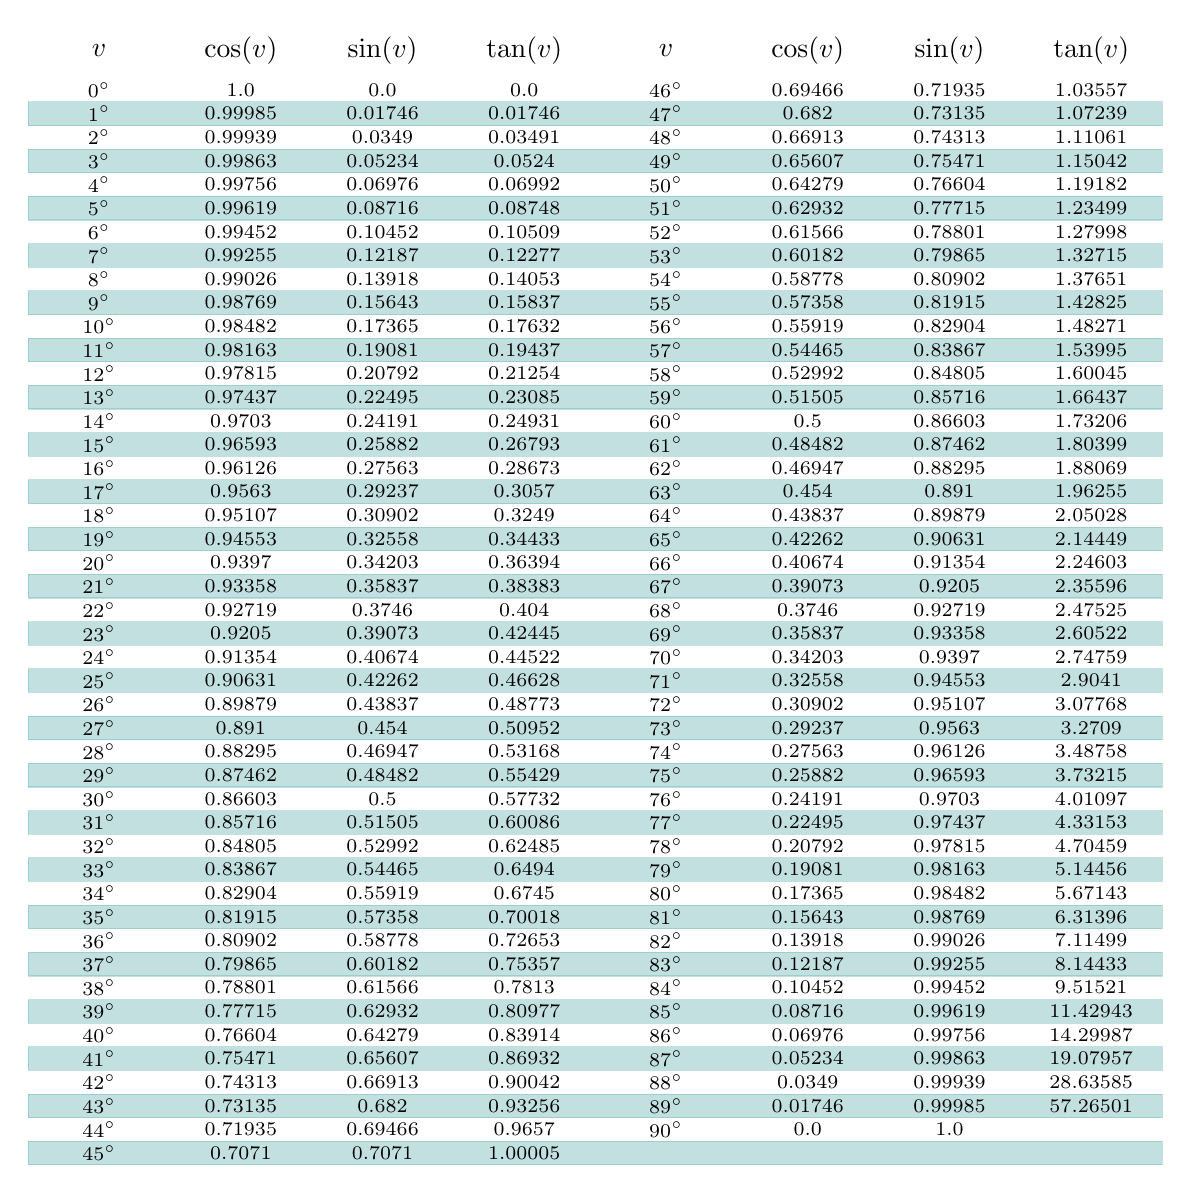
\begin{tikzpicture}
	\node at (0,0) {$v$};
	\node at (2*0.9,0) {$\cos(v)$};
	\node at (4*0.9,0) {$\sin(v)$};
	\node at (6*0.9,0) {$\tan(v)$};
	\node at (8*0.9,0) {$v$};
	\node at (10*0.9,0) {$\cos(v)$};
	\node at (12*0.9,0) {$\sin(v)$};
	\node at (14*0.9,0) {$\tan(v)$};
	\scriptsize
	%Colors
	\foreach \i in {0,...,22}{
		\filldraw[color = teal!60, opacity = 0.4] (-0.9,-0.5-0.3+0.15-\i*0.3*2) rectangle
		 (14*0.9 + 0.9,-0.5-0.3-0.15-\i*0.3*2);
	}
	\foreach \i in {0,...,45}{
		%Macros for evaluating
		\pgfmathsetmacro{\cval}{cos(\i)}
		\pgfmathsetmacro{\sval}{sin(\i)}
		\pgfmathsetmacro{\tval}{tan(\i)}
		%First columns of values
		\node at (0,-0.5-\i*0.3) {$\i^{\circ}$};
		\node at (2*0.9,-0.5-\i*0.3) { \cval };
		\node at (4*0.9,-0.5-\i*0.3) { \sval };
		\node at (6*0.9,-0.5-\i*0.3) { \tval };
	}
	\foreach \i in {46,...,89}{
		%Macros
		\pgfmathsetmacro{\cval}{cos(\i)}
		\pgfmathsetmacro{\sval}{sin(\i)}
		\pgfmathsetmacro{\tval}{tan(\i)}
		%Second column
		\node at (8*0.9,-0.5-\i*0.3 + 46*0.3) {$\i^{\circ}$};
		\node at (10*0.9,-0.5-\i*0.3 + 46*0.3) { \cval };
		\node at (12*0.9,-0.5-\i*0.3 + 46*0.3) { \sval };
		\node at (14*0.9,-0.5-\i*0.3 + 46*0.3) { \tval };
	}
		\pgfmathsetmacro{\cval}{cos(90)}
		\pgfmathsetmacro{\sval}{sin(90)}
		\node at (8*0.9,-0.5-90*0.3 + 46*0.3) {$90^{\circ}$};
		\node at (10*0.9,-0.5-90*0.3 + 46*0.3) { \cval };
		\node at (12*0.9,-0.5-90*0.3 + 46*0.3) { \sval };
	\end{tikzpicture}
	\caption{Tabel over udvalgte værdier for $\cos$, $\sin$ og $\tan$.}
	\label{tab:cossintan}
\end{table}

\newpage


\subsection*{Opgave 1}

Bestem arealet af trekant $\triangle ABC$ ved at bruge Tabel \ref{tab:cossintan}.

\begin{center}
	\begin{tikzpicture}
		\draw[color = olive, thick] (-7,0) -- (0,0) node[midway, anchor = south] {$5$};
		\draw[color = olive, thick] (-5.2,-3) -- (0,0) node[midway, anchor = north west] {$6$};
		\draw[color = olive, thick] (-7,0) -- (-5.2,-3) node[midway, anchor = east] {$c$};
		\draw[color = olive, thick] (-0.7,0) arc (180:210:0.7) node[midway, anchor = east] {$30^{\circ}$};
		\node[color = olive, anchor = east] at (-7,0) {$A$};
		\node[color = olive, anchor = west] at (0,0) {$C$};
		\node[color = olive, anchor = north] at (-5.2,-3) {$B$};
	\end{tikzpicture}
\end{center}

\subsection*{Opgave 2 (med hjælpemidler)}

En trekant $\triangle ABC$ har $\angle C = 50$, $a = 10$ og $b = 7$
\begin{enumerate}[label=\roman*)]
	\item Bestem arealet af $\triangle ABC$
\end{enumerate}

\subsection*{Opgave 3 (med hjælpemidler)}
En trekant $\triangle ABC$ har $\angle A = 120$, $b = 5$ og et areal på 19.
\begin{enumerate}[label=\roman*)]
	\item Tegn en skitse af $\triangle ABC$.
	\item Bestem sidelængden $c$. 
\end{enumerate}

\subsection*{Opgave 4}

En trekant $\triangle ABC$ har $\angle C = 53^\circ$, $a = 2$ og $b = 5$.
\begin{enumerate}[label=\roman*)]
	\item Brug Tabel \ref{tab:cossintan} til at bestemme arealet for $\triangle ABC$. Afrund til én decimal. 
\end{enumerate} 


\subsection*{Opgave 5} 
	Brug enhedscirklen til at bevise Sætning \ref{setn:cossin}.

\subsection*{Opgave 6}
	Vi skal i denne opgave bevise Sætning \ref{setn:areal} for $\angle C > 90^{\circ}$. 
	Betragt følgende trekant $\triangle ABC$.
	\begin{center}
	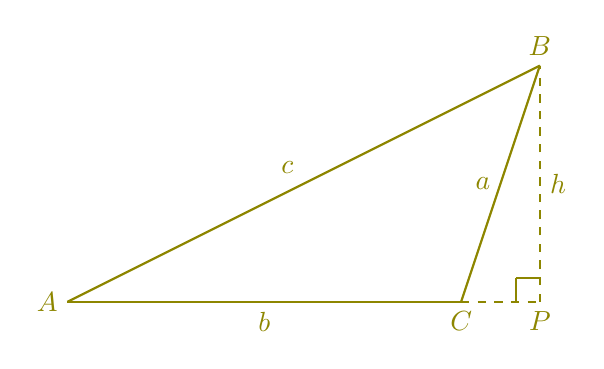
\begin{tikzpicture}
		\draw[color = olive, thick] (0,0) -- (5,0) node[midway, anchor = north] {$b$};
		\draw[color = olive, thick] (0,0) -- (6,3) node[midway, anchor = south east] {$c$};
		\draw[color = olive, thick] (5,0) -- (6,3) node[midway, anchor = east] {$a$};
		\node[color = olive, anchor = east] at (0,0) {$A$};
		\node[color = olive, anchor = north] at (5,0) {$C$};
		\node[color = olive, anchor = south] at (6,3) {$B$};
		\draw[color = olive, thick, dashed] (6,0) -- (6,3) node[midway, anchor = west] {$h$};
		\draw[color = olive, thick, dashed] (5,0) -- (6,0);
		\node[color = olive, anchor = north] at (6,0) {$P$};
		\draw[color = olive, thick] (5.7,0) -- (5.7,0.3);
		\draw[color = olive, thick] (5.7,0.3) -- (6,0.3);
	\end{tikzpicture}
	\end{center}
	\begin{enumerate}[label=\roman*)]
		\item Bevis Sætning \ref{setn:areal} ved brug af denne trekant. (Vink: Anvend sinusformlen på
		 trekant $\triangle BPC$ og fortsæt som i beviset for den spidse vinkel. Husk at udnytte 
		 Sætning \ref{setn:cossin}.)
	\end{enumerate}
\subsection*{Opgave 7}

Vi skal i denne opgave bevise idiotformlen $\cos(v)^2 + \sin(v)^2 = 1$.

\begin{enumerate}[label=\roman*)]
	\item Tegn en retvinklet trekant, hvor hypotenusen er linjestykket fra centrum af enhedscirklen til 
	punktet $P_v$ på kanten af enhedscirklen. 
	\item Hvad er længden af hypotenusen og de to kateter i denne trekant?
	\item Anvend Pythagoras' sætning på denne trekant.
\end{enumerate}

\subsection*{Opgave 8}

Brug idiotformlen til at bestemme $\cos(45)$ eksakt.

\subsection*{Opgave 9}
Vi skal argumentere for, at $\cos(60) = 0.5$. 
\begin{enumerate}[label=\roman*)]
	\item Tegn en enhedscirken med en linje ud til randen af cirklen,
	 der danner en vinkel med $x$-aksen på $60^\circ$.
	\item Tegn en retvinklet trekant, hvor dette er hypotenusen og
	 den hosliggende katete har længden $\cos(60)$.
	\item Hvad er vinklerne i denne trekant?
	\item Kan du tegne en trekant ved siden af denne trekant, der sammen med denne trekant
	 viser at $\cos(60) = 0.5$?
\end{enumerate}
Vi skal nu vise, at $\sin(60) = \frac{\sqrt{3}}{2}$
\begin{enumerate}[label=\roman*)]
	\setcounter{enumi}{4}
\item Indsæt $\cos(60)$ og $\sin(60)$ i idiotformlen og isolér $\sin(60)$. 
\item Kan du argumentere for, at $\sin(30) = 0.5$ og $\cos(30) = \frac{\sqrt{3}}{2}$?
\end{enumerate}

\subsection*{Opgave 10}
Til de følgende to delopgaver skal du bruge Tabel \ref{tab:cossintan}, hvor du afrunder til én decimal.
\begin{enumerate}[label=\roman*)]
	\item Bestem sidelængden $c$ i den første trekant.
	\item Bestem sidelængden $a$ i den anden trekant. 
\end{enumerate}
\begin{center}
	\begin{minipage}{0.45\textwidth}
		\centering
		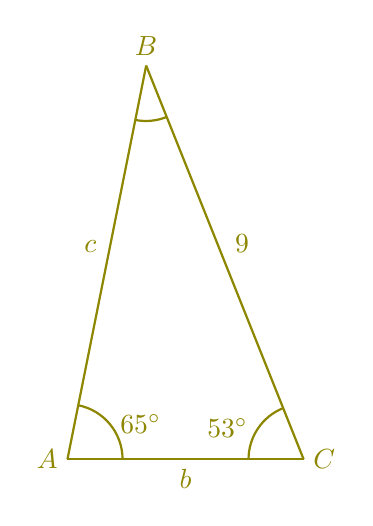
\begin{tikzpicture}
		%A
		\pgfmathsetmacro{\ax}{0}
		\pgfmathsetmacro{\ay}{0}
		%B
		\pgfmathsetmacro{\bx}{1}
		\pgfmathsetmacro{\by}{5}
		%C
		\pgfmathsetmacro{\cx}{3}
		\pgfmathsetmacro{\cy}{0}
		%arc radius
		\pgfmathsetmacro{\arclen}{0.7}
		%c
		\draw[color = olive, thick] (\ax,\ay) -- (\bx,\by) node[midway, anchor = south east] {$c$};
		%b
		\draw[color = olive, thick] (\ax,\ay) -- (\cx,\cy) node[midway, anchor = north] {$b$};
		%a
		\draw[color = olive, thick] (\bx,\by) -- (\cx,\cy) node[midway, anchor = south west] {$9$};
	%	Vinkel A		
		\draw[color = olive, thick] (\arclen,0) arc (0:78.68:\arclen) 
		node[midway, anchor = west] {$65^\circ$};
	%	Vinkel B
		\draw[color = olive, thick] (0.86,4.31) arc (180 + 78.69:180 + 78.69 + 33.11:\arclen)
		 node[midway, anchor = south] {};
	%	Vinkel C
		\draw[color = olive, thick] (\cx - \arclen,0) arc (180:180 - 68.20:\arclen)
		 node[midway, anchor = east] {$53^\circ$};
		 %Nodes
		 \node[color = olive, anchor = east] at (\ax,\ay) {$A$};
		 \node[color = olive, anchor = south] at (\bx,\by) {$B$};
		 \node[color = olive, anchor = west] at (\cx,\cy) {$C$};
		\end{tikzpicture}
	\end{minipage}
		\begin{minipage}{0.45\textwidth}
		\centering
		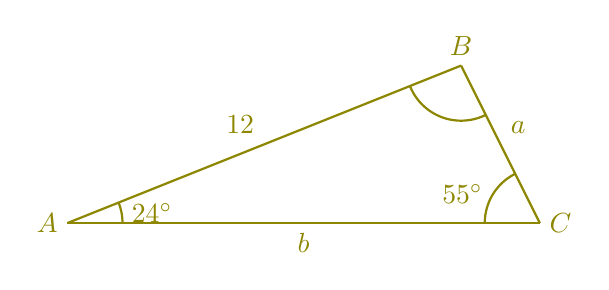
\begin{tikzpicture}
		%A
		\pgfmathsetmacro{\ax}{0}
		\pgfmathsetmacro{\ay}{0}
		%B
		\pgfmathsetmacro{\bx}{5}
		\pgfmathsetmacro{\by}{2}
		%C
		\pgfmathsetmacro{\cx}{6}
		\pgfmathsetmacro{\cy}{0}
		%arc radius
		\pgfmathsetmacro{\arclen}{0.7}
		%c
		\draw[color = olive, thick] (\ax,\ay) -- (\bx,\by) node[midway, anchor = south east] {$12$};
		%b
		\draw[color = olive, thick] (\ax,\ay) -- (\cx,\cy) node[midway, anchor = north] {$b$};
		%a
		\draw[color = olive, thick] (\bx,\by) -- (\cx,\cy) node[midway, anchor = south west] {$a$};
	%	Vinkel A		
		\draw[color = olive, thick] (\arclen,0) arc (0:21.8:\arclen) 
		node[midway, anchor = west] {$24^\circ$};
	%	Vinkel B
		\draw[color = olive, thick] (4.35,1.74) arc (180 + 21.8:180 + 21.8 + 94.76:\arclen)
		 node[midway, anchor = south] {};
	%	Vinkel C
		\draw[color = olive, thick] (\cx - \arclen,0) arc (180:180 - 63.43:\arclen)
		 node[midway, anchor = east] {$55^\circ$};
		 %Nodes
		 \node[color = olive, anchor = east] at (\ax,\ay) {$A$};
		 \node[color = olive, anchor = south] at (\bx,\by) {$B$};
		 \node[color = olive, anchor = west] at (\cx,\cy) {$C$};
		\end{tikzpicture}
	\end{minipage}
\end{center}
\subsection*{Opgave 11}
Til de følgende to delopgaver skal du bruge Tabel \ref{tab:cossintan}, hvor du afrunder til én decimal.
\begin{enumerate}[label=\roman*)]
	\item Bestem $\angle B$ i den første trekant.
	\item Bestem $\angle C$ i den anden trekant. 
\end{enumerate}

\begin{center}
	\begin{minipage}{0.45\textwidth}
		\centering
		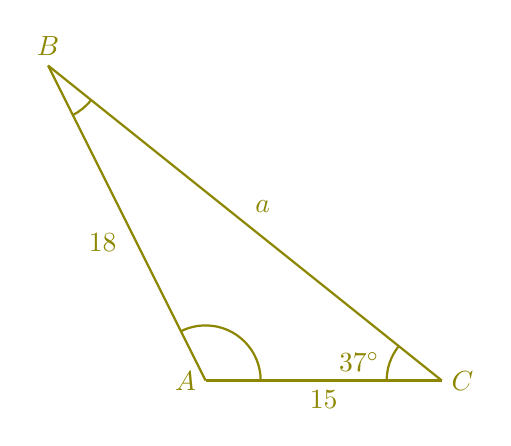
\begin{tikzpicture}
		%A
		\pgfmathsetmacro{\ax}{2}
		\pgfmathsetmacro{\ay}{0}
		%B
		\pgfmathsetmacro{\bx}{0}
		\pgfmathsetmacro{\by}{4}
		%C
		\pgfmathsetmacro{\cx}{5}
		\pgfmathsetmacro{\cy}{0}
		%arc radius
		\pgfmathsetmacro{\arclen}{0.7}
		%c
		\draw[color = olive, thick] (\ax,\ay) -- (\bx,\by) node[midway, anchor = north east] {$18$};
		%b
		\draw[color = olive, thick] (\ax,\ay) -- (\cx,\cy) node[midway, anchor = north] {$15$};
		%a
		\draw[color = olive, thick] (\bx,\by) -- (\cx,\cy) node[midway, anchor = south west] {$a$};
	%	Vinkel A		
		\draw[color = olive, thick] (\ax + \arclen,0) arc (0:116.57:\arclen) 
		node[midway, anchor = west] {};
	%	Vinkel B
		\draw[color = olive, thick] (0.31,3.37) arc (180 + 116.57:180 + 116.57 + 24.78:\arclen)
		 node[midway, anchor = south east] {};
	%	Vinkel C
		\draw[color = olive, thick] (\cx - \arclen,0) arc (180:180 - 38.66:\arclen)
		 node[midway, anchor = east] {$37^\circ$};
		 %Nodes
		 \node[color = olive, anchor = east] at (\ax,\ay) {$A$};
		 \node[color = olive, anchor = south] at (\bx,\by) {$B$};
		 \node[color = olive, anchor = west] at (\cx,\cy) {$C$};
		\end{tikzpicture}
	\end{minipage}
		\begin{minipage}{0.45\textwidth}
		\centering
		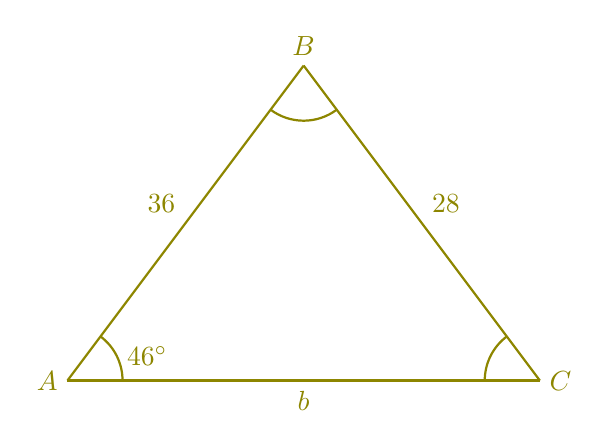
\begin{tikzpicture}
		%A
		\pgfmathsetmacro{\ax}{0}
		\pgfmathsetmacro{\ay}{0}
		%B
		\pgfmathsetmacro{\bx}{3}
		\pgfmathsetmacro{\by}{4}
		%C
		\pgfmathsetmacro{\cx}{6}
		\pgfmathsetmacro{\cy}{0}
		%arc radius
		\pgfmathsetmacro{\arclen}{0.7}
		%c
		\draw[color = olive, thick] (\ax,\ay) -- (\bx,\by) node[midway, anchor = south east] {$36$};
		%b
		\draw[color = olive, thick] (\ax,\ay) -- (\cx,\cy) node[midway, anchor = north] {$b$};
		%a
		\draw[color = olive, thick] (\bx,\by) -- (\cx,\cy) node[midway, anchor = south west] {$28$};
	%	Vinkel A		
		\draw[color = olive, thick] (\ax + \arclen,0) arc (0:53.13:\arclen) 
		node[midway, anchor = west] {$46^{\circ}$};
	%	Vinkel B
		\draw[color = olive, thick] (2.58,3.44) arc (180 + 53.13:180 + 53.13 + 73.74:\arclen)
		 node[midway, anchor = south east] {};
	%	Vinkel C
		\draw[color = olive, thick] (\cx - \arclen,0) arc (180:180 - 53.13:\arclen)
		 node[midway, anchor = east] {};
		 %Nodes
		 \node[color = olive, anchor = east] at (\ax,\ay) {$A$};
		 \node[color = olive, anchor = south] at (\bx,\by) {$B$};
		 \node[color = olive, anchor = west] at (\cx,\cy) {$C$};
		\end{tikzpicture}
	\end{minipage}
\end{center}

\subsection*{Opgave 12 (med hjælpemidler)}
En trekant $\triangle ABC$ opfylder, at $\angle A = 29^\circ$, $\angle B = 55\circ$ og $b = 3$.
\begin{enumerate}[label=\roman*)]
	\item Tegn en skitse af $\triangle ABC$. 
	\item Bestem sidelængden $a$.
\end{enumerate}

\subsection*{Opgave 13 (med hjælpemidler)}
En trekant $\triangle ABC$ opfylder, at $\angle B = 130^\circ$, $b = 50$ og $c = 10$.
\begin{enumerate}[label=\roman*)	]
	\item Tegn en skitse af $\triangle ABC$. 
	\item Bestem vinklen $\angle C$. 
\end{enumerate}

\subsection*{Opgave 14}
Vi skal bevise Sætning \ref{setn:sinusrelation}.
\begin{enumerate}[label=\roman*)]
	\item Udnyt at arealet $M$ for en vilkårlig trekant $\triangle ABC$ kan skrives på følgende tre måder
	\begin{align*}
		M = \frac{1}{2}ab\sin(\angle C) = \frac{1}{2}ac\sin(\angle B) = \frac{1}{2} bc\sin(\angle A)
	\end{align*}
	og dividér hele ligheden med $\frac{1}{2}abc$.
	\item Forkort udtrykket.
\end{enumerate}